\section{光的电磁理论}
通过麦克斯韦方程我们容易得出电磁场的波动方程
\begin{Equation}[电磁场的波动方程]
    \pdv[2]{\vb*{E}}{t}-u^2\laplacian\vb*{E}=\vb*{0}\qquad
    \pdv[2]{\vb*{H}}{t}-u^2\laplacian\vb*{H}=\vb*{0}
\end{Equation}
在\xref{eq:电磁场的波动方程}中的$u$代表电磁波的波速
\begin{Equation}[电磁波的波速]
    u=\frac{1}{\sqrt{\varepsilon_0\varepsilon_r\mu_0\mu_r}}=\frac{1}{\sqrt{\varepsilon_r\mu_r}}
\end{Equation}
在\xref{eq:电磁波的波速}中的$c=1/\sqrt{\varepsilon_0\mu_0}=3\times 10^{8}\si{m\cdot s^{-1}}$即真空光速。

作为对波动光学的简单讨论，我们不愿意就\xref{eq:电磁场的波动方程}的偏微分方程的求解作任何数学上的分析或计算。但为了对电磁波和光有一个直观的物理图景，我们不加证明的指出，\xref{eq:电磁场的波动方程}在恰当的定解条件下是可以给出我们最熟悉的那类平面波（即以平面为波阵面的波）的解的，而且在这种情况下，由于任意波线上每一点出的$\vb*{E},\vb*{H}$矢量的方向是固定的，我们可以简化的用标量$E,H$来表示，另外若假定波动是\udotcn{单一频率}的（即\udotcn{单色}光），那么我们就有$E,H$波函数
\begin{Equation}[电磁波的波函数]
    E=E_0\cos\qty(\omega t-kz+\phi)\qquad
    H=H_0\cos\qty(\omega t-kz+\phi)
\end{Equation}
其中$E_0,H_0$分别代表电场和磁场的振幅，而$\omega$和$k$分别表示角频率和角波数
\begin{itemize}
    \item 所谓角频率，就是指单位时间内的相位变化。
    \item 所谓角波数，就是指单位距离上的相位变化。
\end{itemize}
\begin{Figure}[电磁波的图示]
    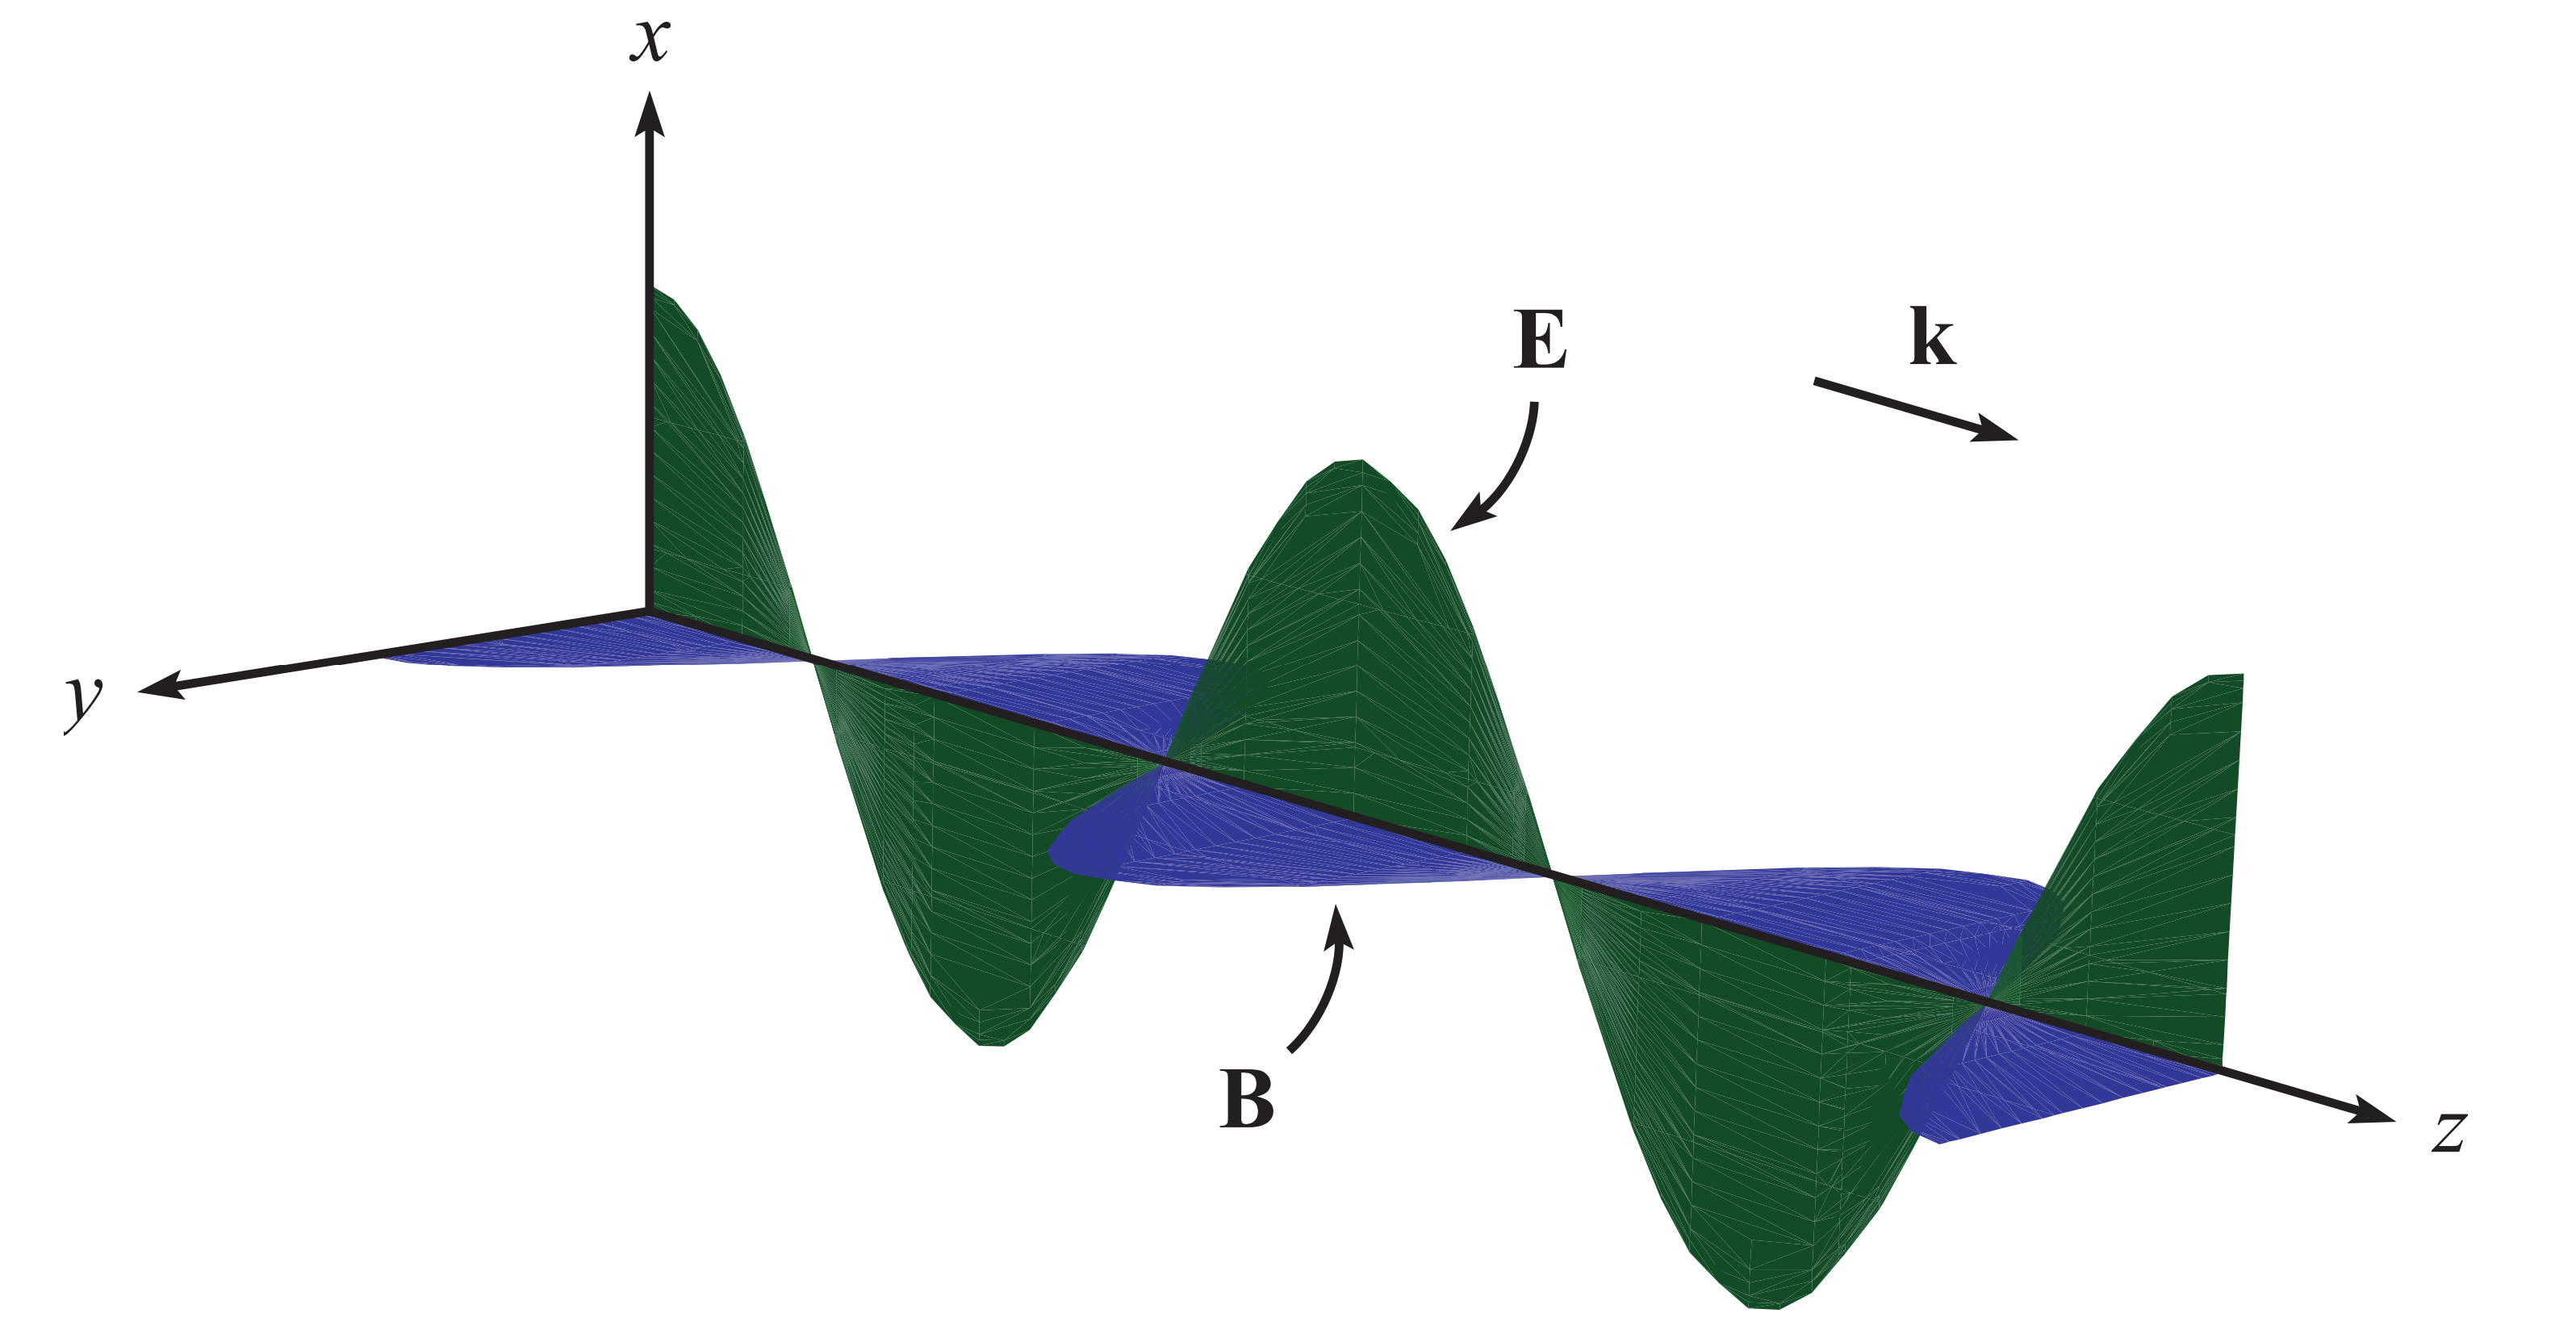
\includegraphics[width=12cm]{image/1.png}
\end{Figure}
除了\xref{eq:电磁波的波函数}的波函数，由\xref{eq:电磁场的波动方程}的求解中还有以下两个重要结论
\begin{enumerate}
    \item 电场强度和磁场强度$\vb*{E},\vb*{H}$的方向总是垂直的，如\xref{fig:电磁波的图示}所示，例如假定波线（即电磁波的传播方向）是沿$z$轴的，那么，矢量$\vb*{E}$就会沿$x$轴方向，矢量$\vb*{H}$就会沿$y$轴方向。
    \item 电场强度和磁场强度的大小之间满足\xref{eq:电场和磁场的代数关系}代数关系。
\end{enumerate}
\begin{Equation}[电场和磁场的代数关系]
    E\sqrt{\varepsilon_0\varepsilon_r}=H\sqrt{\mu_0\mu_r}
\end{Equation}
由此，我们就对光的电磁物理本质有了一定的了解。

\subsection{光强}
通常所说的\uwave{光的强度}或\uwave{光强}，是指光在单位面积上的平均功率，即是光的平均能流密度。\goodbreak

而作为电磁波，此处的能流密度由电磁波的坡印亭矢量给出
\begin{BoxDefinition}[坡印亭矢量]
    \uwave{坡印亭矢量} $\vb*{S}$描述了电磁波的能流密度
    \begin{Equation}
        \vb*{S}=\vb*{E}\times\vb*{H}
    \end{Equation}
    坡印亭矢量指向电场和磁场的右手螺旋方向，故其也表示电磁波的前进方向。
\end{BoxDefinition}
而由于电磁波中$\vb*{E},\vb*{H}$垂直并有$E\sqrt{\varepsilon_0\varepsilon_r}=H\sqrt{\mu_0\mu_r}$，坡印亭矢量的大小$S$为
\begin{Equation}&[1]
    S=\abs{\vb*{E}\times\vb*{H}}=EH=E^2\sqrt{\frac{\varepsilon_0\varepsilon_r}{\mu_0\mu_r}}
\end{Equation}
在光频波段，所有的磁化机制都不起作用，因此可以认为相对磁导率$\mu_r=1$，故
\begin{Equation}&[2]
    S=E^2\sqrt{\frac{\varepsilon_0\varepsilon_r}{\mu_0}}
\end{Equation}
为了进一步简化\xrefpeq{2}，我们引入折射率作为代换变量
\begin{BoxDefinition}[折射率]
    \uwave{折射率} $n$定义为真空光速与介质光速的比
    \begin{Equation}&[]
        n=\frac{c}{u}
    \end{Equation}
\end{BoxDefinition}

\begin{BoxFormula}[折射率与介电常数]
    折射率在近似$\mu_r=1$时是相对介电常数的平方根
    \begin{Equation}&[]
        n=\sqrt{\varepsilon_r}
    \end{Equation}
\end{BoxFormula}
\begin{Proof}
    证明是极为容易的，注意到\xref{eq:电磁波的波速}并代入$\mu_r=1$
    \begin{Equation}*
        n=\frac{c}{u}=c
        \sqrt{\varepsilon_0\varepsilon_r\mu_0\mu_r}=
        \sqrt{\varepsilon_r\mu_r}=\sqrt{\varepsilon_r}\qedhere
    \end{Equation}
\end{Proof}
关于折射率我们再补充一些，我们知道，光或电磁波的本征是频率的，光的频率是恒定值，但是光的波长则有可能随着光传播的介质的变化而变化，波长是被定义为波速和频率的比
\begin{Equation}[真空波长]
    \lambda=\frac{c}{\nu}
\end{Equation}
上式是真空波长$\lambda$，而对于折射率为$n$的介质波长$\lambda_n$，代入$u=c/n$
\begin{Equation}[介质波长]
    \lambda_n=\frac{u}{\nu}=\frac{c}{n\nu}=\frac{1}{n}\lambda
\end{Equation}\nopagebreak
由于折射率$n=\sqrt{\varepsilon_r}>1$，因此\empx{光在介质中的波长总是小于真空波长}。\goodbreak

我们再回到坡印亭矢量，将\fancyref{fml:折射率与介电常数}代入\xrefpeq[坡印亭矢量]{2}
\begin{Equation}
    S=E^2n\sqrt{\frac{\varepsilon_0}{\mu_0}}
\end{Equation}
由于$\sqrt{\varepsilon_0/\mu_0}=\mu_0^{-1}\sqrt{\varepsilon_0\mu_0}=\mu_0^{-1}c^{-1}$
\begin{Equation}
    S=\frac{n}{\mu_0c}E^2
\end{Equation}
这就求出了坡印廷矢量，或者说电磁波的能流密度与电场强度间的关系，这是一个随时间变化的量。但是由于光的频率很高，与我们而言某个时刻的能流密度并没有特别大的意义，我们所关心的光的强度$I$，应该是这种能流密度$S$在时间上的平均值$\xbar{S}$，这将需要用积分表示。
\begin{BoxFormula}[光的强度]
    光的强度$I$表征光的平均能流密度，其与光矢量的平方在时间上的均值成正比
    \begin{Equation}&[]
        I=\xbar{S}=\frac{n}{\mu_0 c}\xbar{E^2}=
        \frac{n}{\mu_0c}\frac{1}{\tau}\Int[0][\tau]{E^2(t)\dd{t}}
    \end{Equation}
\end{BoxFormula}
这里\xrefpeq{}中的$\tau$代表光强$I$是在多长时间上的均值，或者通俗的说就是感光时间。而通常来说光的振动周期是远小于感光时间$\tau$的，也就是说在感光时间$\tau$上光的振动已经重复了足够多的周期了，因此在两侧即便有一些光振动的不完整周期，它们的影响也完全可以忽略了。

这里我们考虑的光作简谐振动，在\xrefpeq{}代入\xrefeq{电磁波的波函数}即得
\begin{Equation}
    I=\frac{n}{\mu_0c}\frac{1}{\tau}\Int[0][\tau]{E_0^2\cos^2(\omega t+\phi)\dd{t}}=\frac{n}{2\mu_0c}E_0^2
\end{Equation}
上式的第二步是基于定积分
\begin{Equation}
    \frac{1}{\pi}\Int[0][\pi]A\cos^2 t\dd{t}=\frac{1}{\pi}\qty(\frac{\pi}{2}A)=\frac{1}{2}A
\end{Equation}
这样我们就求得了简谐光振动的光强
\begin{BoxFormula}[简谐光振动的光强]
    简谐光振动的光强$I$与光矢量振幅$E_0$的平方成正比
    \begin{Equation}
        I=\frac{n}{2\mu_0c}E_0^2
    \end{Equation}
\end{BoxFormula}
以上的\empx{光矢量就是电场强度}，尽管我们说光或电磁波是由电场和磁场的波动共同构成的，但是科学研究表明，光产生的大部分效应，包括视觉的产生，包括感光作用，其中起主要作用的都是电磁波中的电场强度的波动，故称之为\uwave{光矢量}。这也是为何光强用$E_0$而不是$H_0$表示。

\subsection{光程}
在不同介质中，光随时间的相位变化是一定的，也就是说角频率$\omega_n=\omega$，然而在\xref{eq:介质波长}中已经看到，介质波长总小于真空波长，换言之，光随空间的相位变化会随着折射率而改变。

\begin{BoxFormula}[光的介质角频率]
    光在介质中的角频率$\omega_n$，与其在真空中的角频率$\omega$相同
    \begin{Equation}
        \omega_n=\omega
    \end{Equation}
\end{BoxFormula}

\begin{BoxFormula}[光的介质角波数]
    光在介质中的角波数$k_n$，是其在真空中的角波数$k$的折射率$n$倍
    \begin{Equation}
        k_n=nk
    \end{Equation}
\end{BoxFormula}
\begin{Proof}
    根据角波数的定义和\xref{eq:介质波长}
    \begin{Equation}*
        k_n=\frac{2\pi}{\lambda_n}=\frac{2\pi n}{\lambda}=kn\qedhere
    \end{Equation}
\end{Proof}

\xref{fml:光的介质角波数}表明，介质将增大光随空间的相位变化速度，或者说，介质的折射率的意义就是介质角波数和真空角波数的比。因此，对于同一束光，介质中两点间相对于真空相同距离的两点间将具有更大的相位差，诚然，这在实质上因为两者角波数的差异，但是我们也可以等效的将其归因为介质中的两点对于光而言具有更大的距离，这种等效的距离称为\uwave{光程}，很显然的
\begin{BoxFormula}[光程]
    光程被定义为折射率与距离$s$之积，记作$\Delta$
    \begin{Equation}
        \Delta=nr
    \end{Equation}
    光程的物理意义是，在介质中距离为$r$两点间的相位差等效的真空距离。
\end{BoxFormula}
当我们使用光程$\Delta$而不是实际的距离$r$表示“空间”时，无论是介质还是真空，我们都可以使用完全相同的真空角频率$\omega$和真空角波数$k$，这也就是我们引入光程$\Delta$的积极意义所在。

